\documentclass[12pt, a4paper]{article}

\setlength{\parskip}{.3em}
\setlength{\parindent}{2em}

\usepackage{mathtools}
\usepackage{amssymb}
\usepackage{blindtext}
\usepackage{graphicx}
\usepackage{float}
\usepackage{xeCJK}

\xeCJKsetup{CJKglue=\hspace{0pt plus .08 \baselineskip }}
\xeCJKsetup{RubberPunctSkip=false}
\xeCJKsetup{PunctStyle=plain}
\xeCJKsetup{CheckSingle=true}
\setCJKmainfont{Noto Serif CJK TC}[
	FontFace={el}{n}{* ExtraLight},
	FontFace={l}{n}{* Light},
	FontFace={m}{n}{* Medium},
	FontFace={sb}{n}{* SemiBold},
	FontFace={b}{n}{* Bold},
	FontFace={eb}{n}{* Black}
]
\setCJKsansfont{Noto Sans CJK TC}[
	FontFace={el}{n}{* Thin},
	FontFace={l}{n}{* Light},
	FontFace={sl}{n}{* DemiLight},
	FontFace={m}{n}{* Medium},
	FontFace={b}{n}{* Bold},
	FontFace={eb}{n}{* Black}
]
\setCJKmonofont{Noto Sans Mono CJK TC}[
	FontFace={b}{n}{* Bold}
]

\title{Hello, \LaTeX\ World}
\author{nevikw39}

\begin{document}


\maketitle

\begin{abstract}
This is my first \textsf{\textbf{\TeX}} document. I'm definitely obsessed with the astonishing typesetting language. Grand appreciation of professor Donald E. Knuth.
\end{abstract}

\tableofcontents
\listoftables
\listoffigures

\section{hello, world}

This is my first \textsf{\textbf{\TeX}} document.

\section{CJK Fonts}

使用 Google 及 Adobe 合作開發的開源字型家族 Noto。

\begin{table}[H]
    \centering
    \begin{tabular}{l|l}
        ExtraLight & {\fontseries{el}\selectfont 中文} \\ \hline
        Light      & {\fontseries{l}\selectfont 中文}  \\ \hline
        Medium     & {\fontseries{m}\selectfont 中文}  \\ \hline
        Semibold   & {\fontseries{sb}\selectfont 中文} \\ \hline
        Bold       & {\fontseries{b}\selectfont 中文}  \\ \hline
        Black      & {\fontseries{eb}\selectfont 中文} \\
    \end{tabular}
    \caption{CJK Main fonts}
\end{table}

\begin{table}[H]
    \centering\sffamily
    \begin{tabular}{l|l}
        Thin      & {\fontseries{el}\selectfont 中文} \\ \hline
        Light     & {\fontseries{l}\selectfont 中文}  \\ \hline
        DemiLight & {\fontseries{sl}\selectfont 中文} \\ \hline
        Medium    & {\fontseries{m}\selectfont 中文}  \\ \hline
        Bold      & {\fontseries{b}\selectfont 中文}  \\ \hline
        Black     & {\fontseries{eb}\selectfont 中文} \\
    \end{tabular}
    \caption{CJK Sans fonts}
\end{table}

\begin{table}[h]
    \centering\ttfamily
    \begin{tabular}{l|l}
        Medium & {\fontseries{m}\selectfont 中文} \\ \hline
        Bold   & {\fontseries{b}\selectfont 中文} \\
    \end{tabular}
    \caption{CJK Mono fonts}
\end{table}

\section{《周易·謙卦》}

\begin{figure}[h]
    \centering
	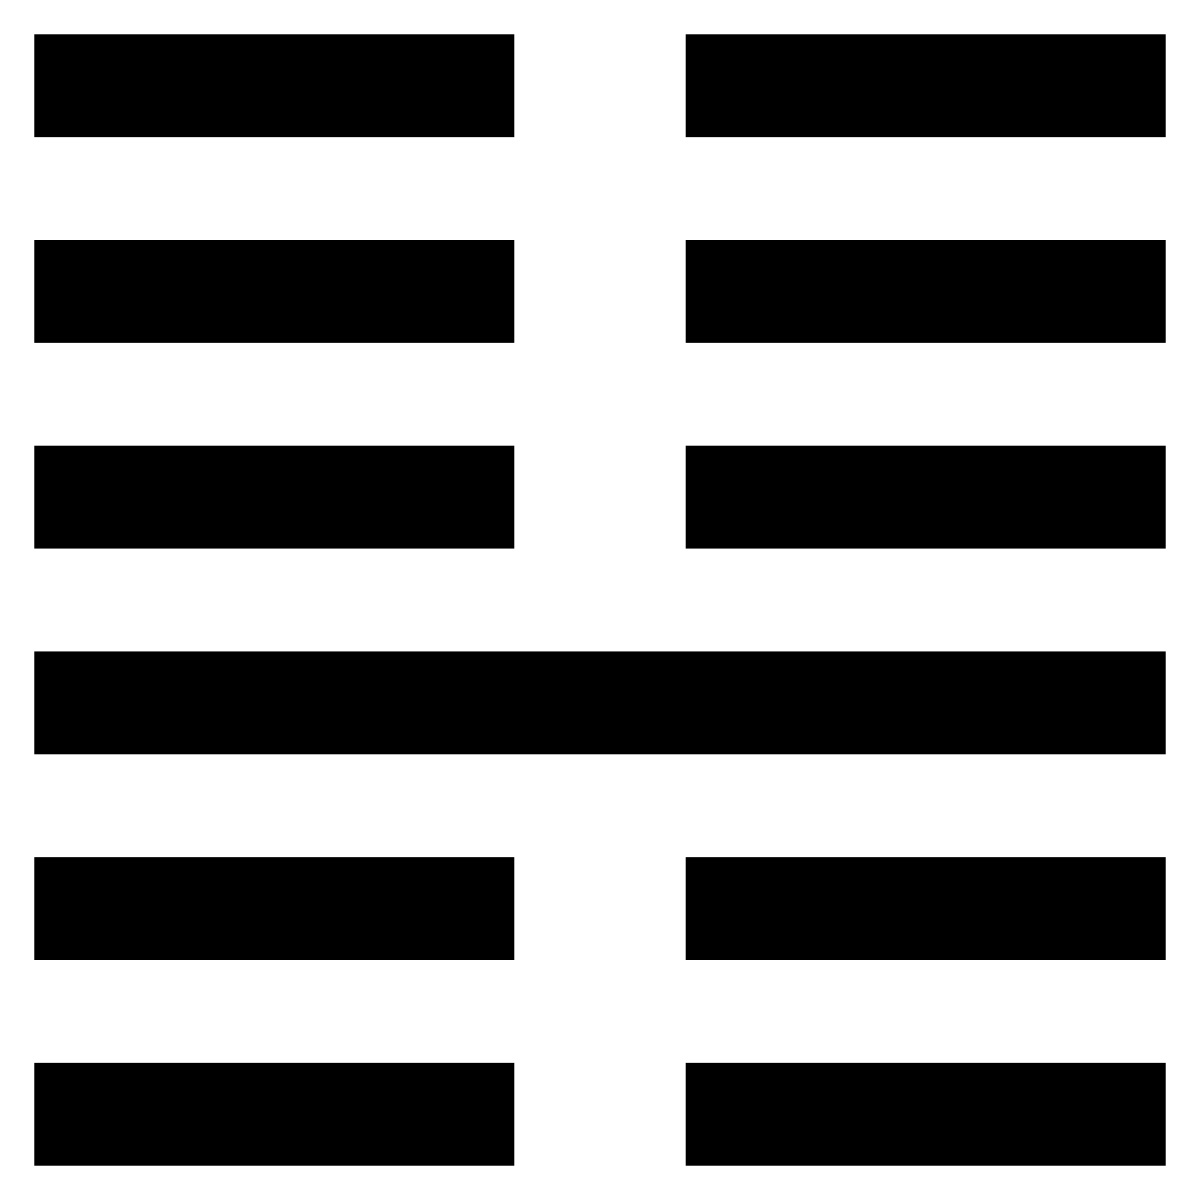
\includegraphics[width=\textwidth/8]{chiang.png}
	\caption{謙卦}
\end{figure}

亨,君子有終。

\subsubsection{彖傳}

謙,亨,天道下濟而光明,地道卑而上行。天道虧盈而益謙,地道變盈而流謙,鬼神害盈而福謙,人道惡盈而好謙。謙尊而光,卑而不可踰,君子之終也。

\subsubsection{象傳}

地中有山,謙;君子以裒\marginpar{裒,音ㄆㄡˊ,減少}多益寡,稱物平施。

\subsection{初六}

謙謙君子,用涉大川,吉。

\subsubsection{象傳}

謙謙\textsf{君}子,卑以自\textsf{牧}也。\footnote{《諫太宗十思疏》:「念高危,則思謙沖而自牧。」}

\subsection{六二}

鳴謙,貞吉。

\subsubsection{象傳}

鳴謙貞吉,中心得也。

\subsection{九三}

勞謙,君子有終,吉。

\subsubsection{象傳}

勞謙君子,萬民服也。

\subsection{六四}

无不利,撝\marginpar{撝,音ㄏㄨㄟ,謙讓}謙。

\subsubsection{象傳}

无不利,撝謙;不違則也。

\subsection{六五}

不富,以其鄰,利用侵伐,无不利。

\subsubsection{象傳}

利用侵伐,征不服也。

\subsection{上六}

鳴謙,利用行師,征邑國。

\subsubsection{象傳}

鳴謙,志未得也。可用行師,征邑國也。

\section{Fabonacci Sequence}

\[F_0 = 0\]
\[F_1 = 1\]
\[F_n = F_{n-1} + F_{n-2}\ (n \geq 2)\]

\subsection{Martix}

Let $Fib(n) = \begin{bmatrix} F_n & F_{n-1}\end{bmatrix}$.\\[1cm]
Given $Fib(n) = base \times Fib(n-1)$.\\[1em]
Then $base = \begin{bmatrix} 1 & 1 \\ 1 & 0\end{bmatrix}$.\\
Therefore, $Fib(n) = \begin{bmatrix} 1 & 1\end{bmatrix} \times \begin{bmatrix} 1 & 1 \\ 1 & 0\end{bmatrix}^{n-2}$.\\[10pt]
With \textsl{binary exponentiation}, we can compute \textit{Fabonacci Number} in $\Theta(\log n)$.

\section{模逆元}

逆元\textit{(Inverse Element)}、逆元素,又稱反元素,是加法相反數與乘法倒數的推廣。對於一元素及一二元運算,若存在一元素與前者進行運算後可得\textbf{單位元素},則稱後者為前者之\textbf{「逆元」}。

模逆元,通常專指模運算中的乘法逆元\textit{(Modular Multiplicative Inverse)}。對於整數 $a,\ b$,若整數 $x$ 滿足 $ax \equiv 1 \pmod b$,則稱 $x$ 為 $a$ 關於 $b$ 之模逆元,記作 $x = a^{-1}$。

在模運算下,加法、減法及乘法遵守分配律。舉例而言:\[87 + 69 \equiv 1 \equiv (87 \bmod 5) + (69 \bmod 5) \pmod 5\]\[87 - 69 \equiv 3 \equiv (87 \bmod 5) - (69 \bmod 5) \pmod 5\]\footnote{在數學中,模運算的結果就是取歐幾里得除法的餘數。關於負數的模,一般來說,數論總是使用正餘數。然而,對於不同的程式語言、編譯器或標準,在實作上或許有不同。D. E. Knuth 教授在 TAOCP 定義 $q = \lfloor\frac{a}{n}\rfloor$ 總是向下取整,即使商是負數,因此餘數和除數有一致符號。}\[87 \times 69 \equiv 3 \equiv (87 \bmod 5) \times (69 \bmod 5) \pmod 5\] 但是,$56 \div 7 \equiv 3 \pmod 5$ 而 $(56 \bmod 5) \div (7 \bmod 5) \equiv 0 \pmod 5$ 顯然不合。一般運算中,若要計算 $56 \div 7$ 相當於計算 56 乘以 7 之倒數;類似地,若要計算 $56 \div 7 \pmod 5$ 則相當於計算 56 乘以 7 之模逆元 3$(\because  7 \times 3 \equiv 1 \pmod 5)$,即 $56 \div 7 \equiv 3 \equiv 56 \times 3 \pmod 5$。

模逆元並非總是存在。若且唯若 $a$ 與 $p$ 互質則 $a^{-1}$ 有意義。

\subsection{求冪}

根據「費馬小定理\textit{(Fermat's little theorem)}」,對於一整數 $a$ 及一質數 $p$,我們有:
\[a^p \equiv a \pmod p\]
等式兩邊同除以 $a^2$,可得:
\[a^{p-2} \equiv a^{-1} \pmod p\]
故可利用快速冪求之。

\subsection{解線性同餘方程式}

當題目所給之模 $n$ 非質數,則吾人即無法透過費馬小定理計算模逆元,此時回到原式。

對於 $ax \equiv 1 \pmod b$ 此「線性同餘方程式」,可以「擴展歐幾里得算法」解之。

\subsection{利用歐拉定理}

歐拉定理其實是費馬小定理的衍生,它表明:
\[a^{\phi(n)} \equiv 1 \pmod n\]
其中,$\phi(n)$ 為歐拉函數,表小於 $n$ 且與 $n$ 互質之正整數之個數。等式兩邊同除以 $a^2$,可得:
\[a^{\phi(n)-1} \equiv a^{-1} \pmod n\]

\section{Blind}

\subsection{Text}

\blindtext

\subsection{Itemize}

\blinditemize[5]

\subsection{Enum}

\blindenumerate[5]

\subsection{Description}

\blinddescription[5]

\subsection{Math}

\blindmathpaper

\end{document}
